\documentclass[12pt]{article}
\usepackage{graphicx}
\usepackage[margin=0.8in]{geometry}
\begin{document}
{\bf Names:} Jack Bracewell, Milan Misak, Craig Ellis \\
{\bf Usernames:} jb2910, mm5510, ce710 \\
{\bf Group Number: 28}  \\ \\

\section*{Assignment 4: Case Based Reasoning}

\subsubsection*{How did you solve the problem of finding two or more best matches with different labels in function RETRIEVE?}

In \emph{retrieve} we iterate over all the cases and calculate similarity of each case and the one passed into the function. We store the value of the highest similarity we found so far and an array of cases which had that similarity. Then for each emotion we calculate the sum of typicalities of cases from our array. Then we return the first case whose emotion is the one with the highest total typicality.


\subsubsection*{Discuss what happens if you try to add a case to CBR system that is already there (either initialisation phase or when you call the retain function? How did you deal with this issue?}

We just increment the typicality of the case that is already in the CBR system and discard the new case. 

\subsubsection*{Compare the different similarity measures you have used (at least three). What are the advantages/disadvantages of each measure?}

The first similarity measure we used was the size of the intersection of 2 AU vectors, normalised. This method was quite quick but only resulted in a classification rate of 73.2. \\ 

We also used the Jaccard Index and Dice coefficient (used to measure the similarity of 2 sets) as measures, these had surprisingly the same $F_1$ measure of: 77.5. Whilst still being relatively quick due to not needing to be normalised.\\

The final similarity measure we tried was a normalised Levenshtein Distance between 2 problems, it is normaly used to compare strings to provide correction suggestions in spellcheckers, because the AU Vector always had the same ordering we could use it to compare their similarity. It was so slow that we do not have cross validation results for it using our K-NN method. For comparison, Dice's classification rate using our faster System (which involved calculating average AU vectors for each category, so only 6 similarities needed to be calculated as opposed to once for each case) was: 42.2 Jaccard's: 50.5 and Levenshtein was 43.3. The Cross Validation forLevenshtein took minutes compared to a couple of seconds for the other similarity measures.  \\ \\

\subsubsection*{Describe how you initialise your CBR system.}

Our CBR system is fairly simple as it only consists of a cell array of cases. To initialise it we iterate over examples in the given clean data creating a case for each example on the fly. For every case we check if the CBR system already contains an equal case and if so then we increment typicality of the already stored case otherwise we add the new case to the CBR system.

\subsubsection*{CBR belongs to a specific class of learning algorithms?! How are these algorithms called and what are the differences with other learning algorithms, like neural networks and decision trees?}
%TODO: that first sentence isn't even a question... I've put an exclamation mark there to see if anyone notices

Online learning algorithms. The difference is that for online algorithms the learning never ends. Their performance should be continually improved with every new case they encounter. Offline learning algorithms do not continue learning once the training is completed.


\subsection*{Implementation details}
\begin{itemize}
  \item RETRIEVE:
    We Cycle through all the cases in the structure, picking the cases with the 3 highest similarities to the case we are attempting to classify (3-NN). If there are more than 3 with the same similarity then they are included in the "voting" not discarded.
  \item REUSE:
    We simply assign the solution value from the retrieved case to the case we are classifying.
  \item RETAIN:
    A new case is made with the corrosponding AU Vector and solution that was found. The weight is value used for calculating similarity is set to 0.8 because that is roughly the classification rate, ie - how much we should trust the prediction opposed to the training data which we know is correct.
  \item CBR cases:
    Each case has an AUVector, a solution and a typicality value, the use of which is explained previously
\end{itemize}


\subsection*{Evaluation results}

\begin{table}
\centering
\begin{tabular}{r r | r r r r r r}
\multicolumn{8}{c}{Predicted class} \\
&  & Anger & Disgust & Fear & Happiness & Sadness & Surprise \\
\hline
 & Anger            & 9.9 & 1.0  & 0.5 & 0.4  & 1.2 & 0.2  \\
 & Disgust          & 0.9 & 16.5 & 0.5 & 0.6  & 1.2 & 0.1  \\
Actual class & Fear & 0.4 & 0.3  & 9.5 & 0.3  & 0.3 & 1.1  \\
 & Happiness        & 0   & 0.6  & 0.3 & 19.9 & 0.4 & 0.4  \\
 & Sadness          & 1.0 & 2.0  & 0.4 & 0.3  & 9.1 & 0.4  \\
 & Surprise         & 0   & 0.1  & 0.7 & 0.5  & 0.3 & 19.1 \\
\end{tabular} 
\caption{Confusion matrix}
\end{table}

\begin{table}
\centering
\begin{tabular}{l | r r}
Emotion & Recall rate (\%) & Precision rate (\%) \\
\hline
Anger     & 75.0000 & 81.1475 \\
Disgust   & 83.3333 & 80.4878 \\
Fear      & 79.8319 & 79.8319 \\
Happiness & 92.1296 & 90.4545 \\
Sadness   & 68.9394 & 72.8000 \\
Surprise  & 92.2705 & 89.6714 \\
\end{tabular}
\caption{Recall and precision rates}
\end{table}

\begin{table}
\centering
\begin{tabular}{l | r}
Emotion & \( F_1 \) measure \\
\hline
Anger     & 77.9528 \\
Disgust   & 81.8859 \\
Fear      & 79.8319 \\
Happiness & 91.2844 \\
Sadness   & 70.8171 \\
Surprise  & 90.9524 \\
\end{tabular}
\caption{F1 measures}
\end{table}

Average classification rate = 0.8367 \\ \\
Confusion matrix: the confusion matrix suggests that our neural networks work well. Anger, disgust and sadness are sometimes classified incorrectly as some other emotion from this group. Otherwise the predicted emotions work very well and some misclassifications do not occur at all (or haven't occurred during our testing). For example happiness has never been classified as anger. Classification rate: this is very high as it normally reaches over 80 per cent whenever we run the program. It is a lot higher than last time when we were using decision trees. It also means that our classifier is very precise and reliable. Recall/precision rate: these are very similar for most emotions. Sadness was slightly harder to recognise. Happiness is also worth mentioning as it was very nearly all the time (93 per cent) recognised. Once it was recognised it was done so correctly with a slightly lower probability. The $F_1$ measure confirms what we have already seen which is that happiness and surprise are classified very well while sadness is the one with most classification errors.


\newpage
\subsection*{Code Flowchart}

TODO
%\begin{center}
%  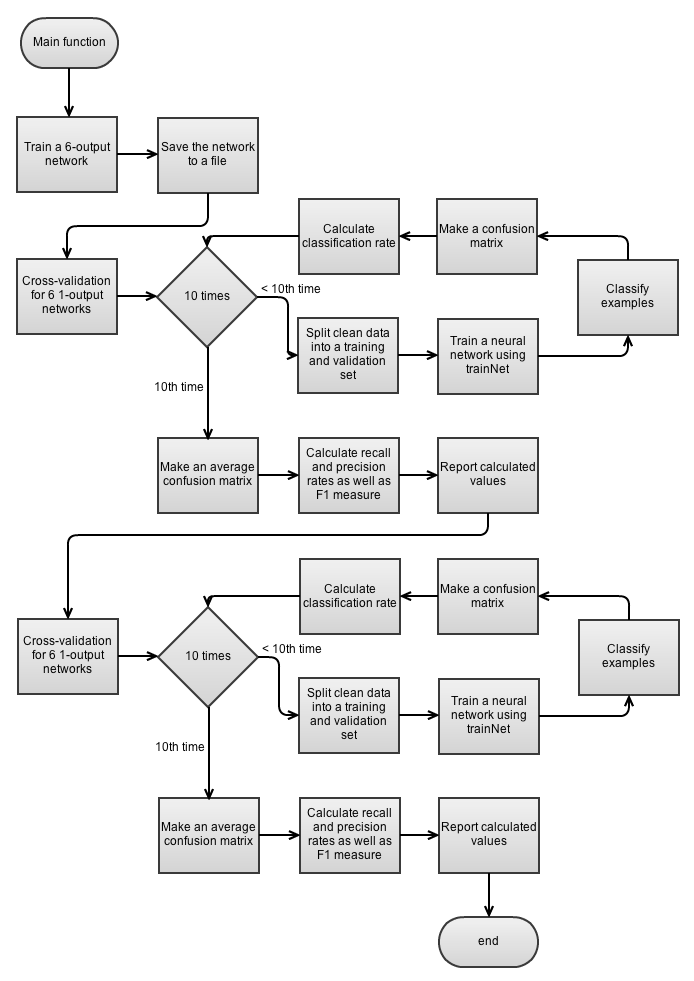
\includegraphics[scale=0.7]{report-images/main.png}
%\end{center}



\end{document}
